\documentclass[tikz]{standalone}

\begin{document}
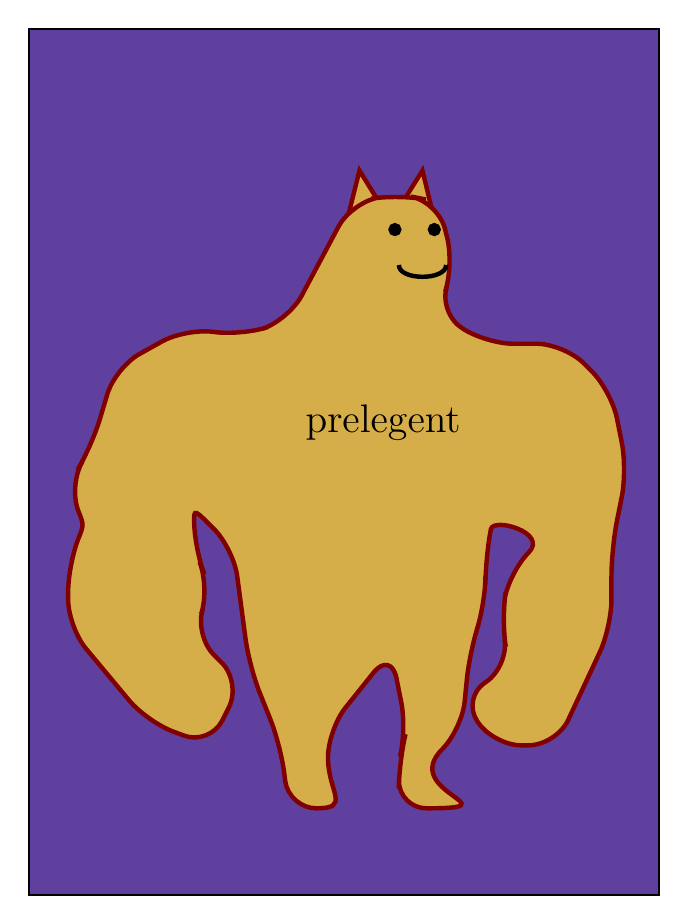
\begin{tikzpicture}[thick]

\draw[fill=blue!50!brown] (-2,-3) rectangle (6,8);

% % Ears
\draw[ red!50!black, ultra thick, fill=yellow!30!brown] (3,6.2) -- ++(-0.5,-0.8) arc[start angle=30+180, end angle=150+180, radius=0.4cm] -- cycle;
\draw[ red!50!black, ultra thick, fill=yellow!30!brown] (2.2,6.2)-- ++(-0.2,-0.8) arc[start angle=30+180, end angle=150+180, radius=0.4cm] -- cycle;

% Shoulders and Chest
\draw[rounded corners=10pt, red!50!black, ultra thick, fill=yellow!30!brown] (0,4.2) -- ++(-0.9,-0.5) --++(-0.3,-1) -- ++(-0.3,-0.5)  .. controls ++(0.2,-0.5) .. ++ (0,-1) --++ (0,-.8) --++ (1,-1.2) --++ (0.8,-0.3) --++ (0.4,0.8) --++ (-.6,.6) --++ (.2,.6) --++ (-.2,.5)  .. controls ++(0,.5) ..++ (.5,0) --++ (.2,-1.5) --++ (.4,-1) --++ (.1,-.8) .. controls ++(.8,0) and ++(0,-0.8) ..++ (.5,1) --++ (0.8,1) --++ (0.2,-1) --++ (-0.1,-0.4) --++ (0,-0.6) .. controls ++(1.5,0) and ++(-.8,-0.8) ..++ (0.8,1) --++ (0.1,1) --++ (0.2,0.6) --++ (0,0.6) .. controls ++(0.1,0.5) and ++(0.5,0.5) .. ++ (0.3,-0.2) --++ (-.1,-.6) --++ (.1,-.6) --++ (-.6,-.4) --++ (.4,-.6) --++ (.8,0) --++ (.7,1.5) --++ (0,1) --++ (.2,1) --++ (-.2,1) --++ (-.6,.6) --++ (-1,0) --++ (-.6,.4) --++ (.2,.6) --++ (-.2,.8) --++ (-.5,.1) --++ (-.6,-.1) --++ (-.8,-1.5) --++ (-.6,-.2) --cycle

  ;

% face

\draw[thick, fill=black] (2.65,5.45) circle (0.07);
\draw[thick, fill=black] (3.15,5.45) circle (0.07);
\draw[ultra thick] (2.7,5) .. controls ++(0,-.2) and ++(0,-.2) ..++ (0.6,0);


\node at (2.5,3) {\Large prelegent};


\end{tikzpicture}
\end{document}
